\section{A first image}\label{sec:first-image}

Because nothing absorbs or scatters, a thermal gravitational image is a line
integral. Integrating Eq.~\eqref{eq:kirchhoff} over frequency for constant
$\eta$ gives the energy emitted per unit volume and solid angle,
$j_E = \alpha\sigma T^4/\pi$, where $\sigma$ is the Stefan--Boltzmann constant.
Dividing by the mean energy of a thermal quantum, $2.70\,\kB T$, gives a
number emissivity $j_N$, and the brightness of the pixel that looks along the
unit vector $\hat n$ is
\begin{equation}\label{eq:column}
N(\hat n) = \int_0^\infty j_N\bigl(s\,\hat n\bigr)\,\dd s ,
\end{equation}
in gravitons per second, per square metre of aperture, per steradian. Every
body along the line of sight contributes, whatever lies in front of it.

Figure~\ref{fig:sun-at-midnight} evaluates Eq.~\eqref{eq:column} for an
observer on the night side of the Earth. In light, the ground is opaque. In
thermal gravitational radiation the planet is a set of nested glowing shells,
brightest where the line of sight is longest and the rock hottest, and the
Sun's core shines through it. The Sun radiates of order $10^{8}\,\mathrm{W}$ in
gravitational waves \cite{GarciaCelyRingwald2025,Steane2024}, about
$4\times10^{-16}\,\mathrm{W\,m^{-2}}$ at the Earth: roughly one graviton per
square metre per second. That is some $10^{10}$ times the surface brightness
of the Earth's interior in this model, so the Sun dominates the thermal
gravitational sky by day and by night.

\begin{figure}
\centering
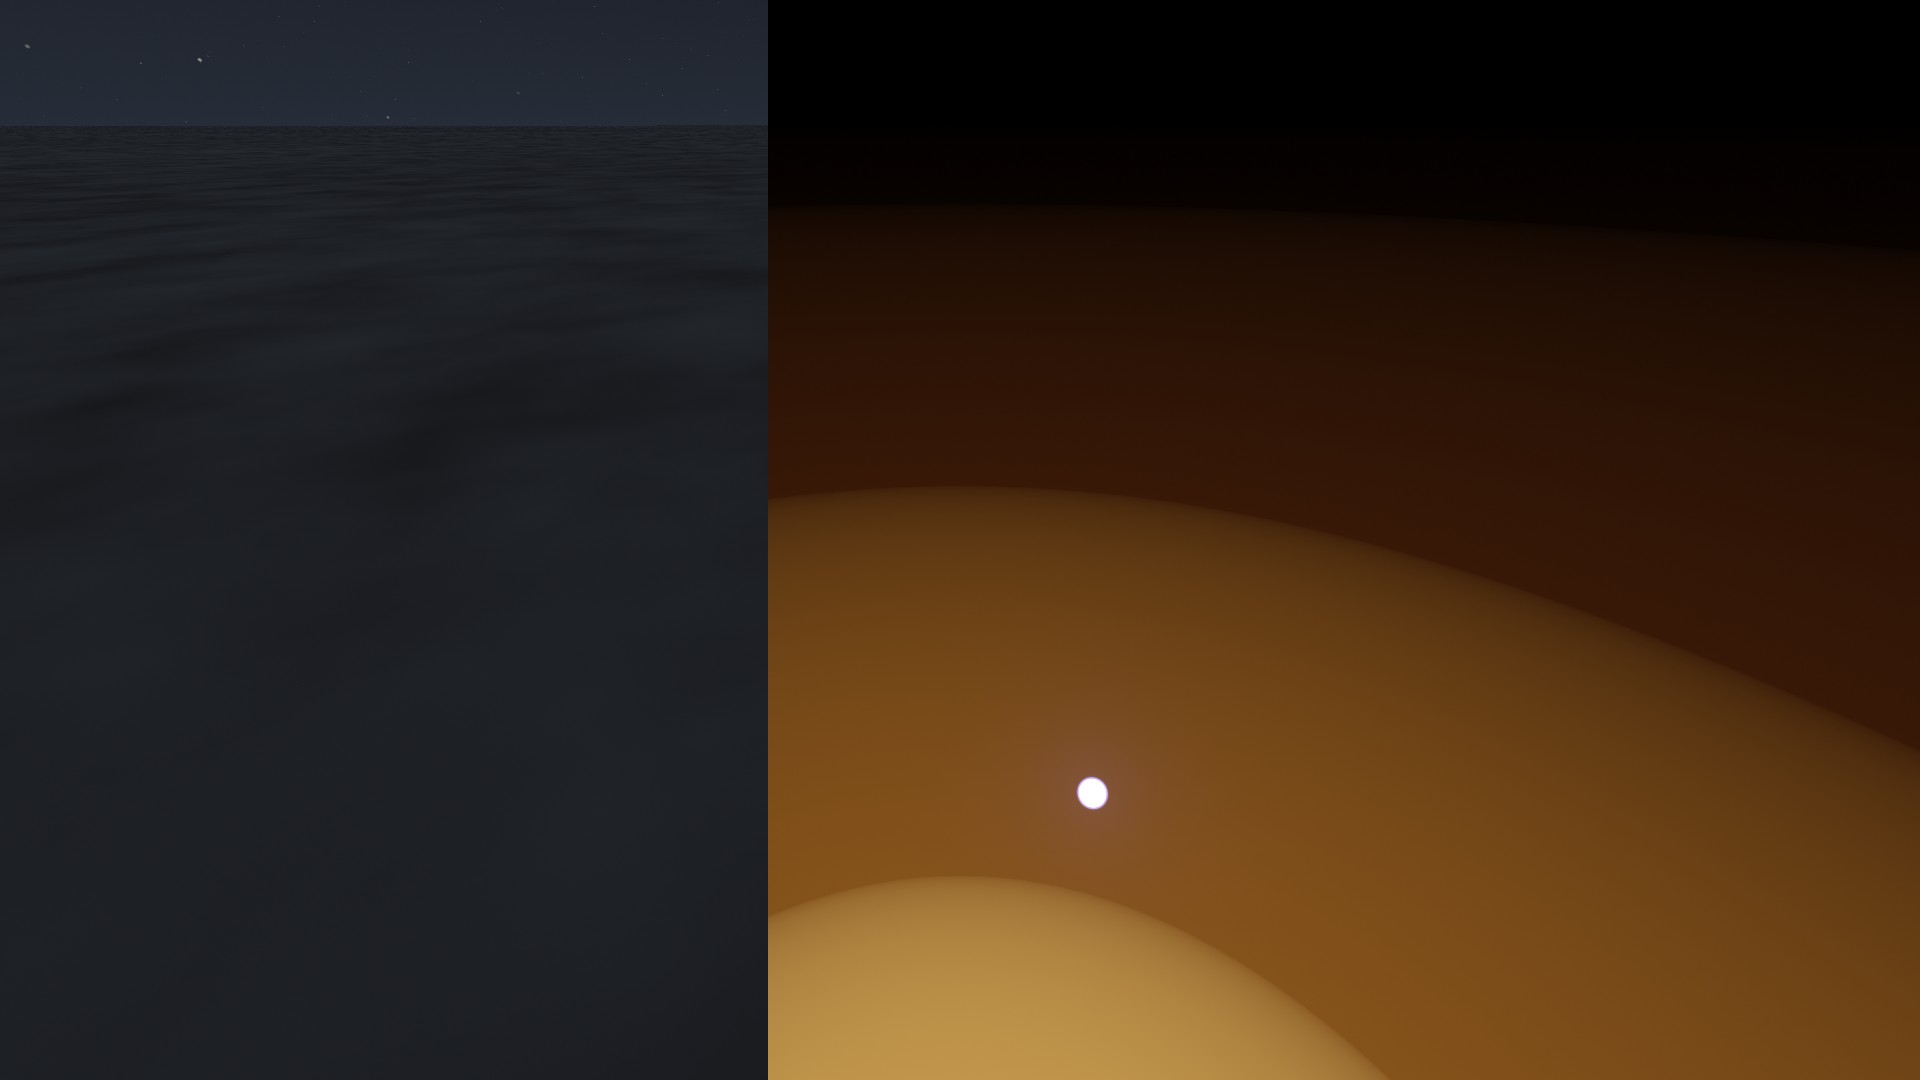
\includegraphics[width=\linewidth]{figures/sun-at-midnight.jpg}
\caption{The Sun at midnight. Left: ordinary light. Right: the expected thermal
gravitational image, Eq.~\eqref{eq:column}, with colour standing for source
temperature. The Earth's internal friction is an assumed placeholder
($\eta = 10^{-3}\,\mathrm{Pa\,s}$ throughout), and the Sun's emission is spread
uniformly over the inner fifth of its radius.}\label{fig:sun-at-midnight}
\end{figure}

The image is an expectation value. At these rates a perfect detector would
register single gravitons, and the picture would assemble itself over hours for
the Sun and far longer for anything else.
